\documentclass{article}
\usepackage{arxiv}
\usepackage[utf8]{inputenc} % allow utf-8 input
\usepackage[T1]{fontenc}    % use 8-bit T1 fonts
\usepackage{hyperref}       % hyperlinks
\usepackage{url}            % simple URL typesetting
\usepackage{booktabs}       % professional-quality tables
\usepackage{amsfonts}       % blackboard math symbols
\usepackage{nicefrac}       % compact symbols for 1/2, etc.
\usepackage{microtype}      % microtypography
\usepackage{lipsum}
\usepackage{graphicx}
\usepackage{float}

\title{\textbf{Simulación de una Ruleta} \\ \large Trabajo Práctico 1.1}
\author{
 Dedich Santiago \\
  Universidad Tecnológica Nacional - FRRO\\
  Zeballos 1341, S2000, Argentina\\
  \texttt{santidedich3226@gmail.com} \\
   \And
 Salami Tomás \\
  Universidad Tecnológica Nacional - FRRO\\
  Zeballos 1341, S2000, Argentina\\
  \texttt{tomas.salami1@gmail.com} \\
  \And
Mesapelle Giani\\
  Universidad Tecnológica Nacional - FRRO\\
  Zeballos 1341, S2000, Argentina\\
  \texttt{gianimesapelle04@gmail.com}\\
  \And
Lovatti Francisco\\
  Universidad Tecnológica Nacional - FRRO\\
  Zeballos 1341, S2000, Argentina\\
  \texttt{franciscolovatti08@gmail.com}\\
  %% \AND
  %% Coauthor \\
  %% Affiliation \\
  %% Address \\
  %% \texttt{email} \\
  %% \And
  %% Coauthor \\
  %% Affiliation \\
  %% Address \\
  %% \texttt{email} \\
  %% \And
  %% Coauthor \\
  %% Affiliation \\
  %% Address \\
  %% \texttt{email} \\
}
\date{Mayo 2026}
\begin{document}

\maketitle

\begin{abstract}
El presente trabajo tiene como objetivo desarrollar una simulación computacional del funcionamiento de una ruleta de casino europea utilizando Python. Se evalúa estadísticamente el comportamiento del juego mediante el análisis de frecuencias absolutas y relativas, y se representan gráficamente los resultados obtenidos.\\
\textbf{Palabras clave:} simulación, ruleta, Python, análisis estadístico, probabilidad.
\end{abstract}

\section{Introducción}
La ruleta es uno de los juegos de azar más populares en los casinos de todo el mundo. Su funcionamiento se basa en un disco giratorio con 37 casillas numeradas del 0 al 36, donde una bola lanzada puede detenerse al azar en cualquiera de ellas. Con este trabajo, utilizaremos Python para simular múltiples tiradas de la ruleta y observar cómo evolucionan diversas métricas estadísticas, como la frecuencia relativa de un número elegido, el promedio, la varianza y el desvío estándar a medida que incrementamos el número de tiradas.

Desde el punto de vista de la Probabilidad y la Estadistica, dado que cada número de la ruleta tiene la misma probabilidad de salir ($1/37$), a medida que el número de observaciones ($N$) tiende a infinito, la variabilidad de los estimadores estadísticos disminuye, convergiendo hacia los parámetros teóricos de una distribución uniforme discreta.  

Llevaremos a cabo varias corridas independientes de la simulación para comparar los resultados obtenidos con los valores teóricos esperados. De este modo, comprobaremos de forma práctica la ley de los grandes números y demostraremos cómo las simulaciones por computadora pueden ayudar a entender mejor el comportamiento de procesos aleatorios.

\section{Conceptos teóricos empleados}
\begin{itemize}
  \item \textbf{Población:} conjunto total de elementos a estudiar. En este trabajo se considera como población teórica el conjunto de todas las tiradas posibles.
  \item \textbf{Muestra:} subconjunto de la población. En este caso, cada conjunto de tiradas simuladas representa una muestra.
  \item \textbf{Frecuencia relativa:} \(f = \frac{n_i}{N}\), donde \(n_i\) es la cantidad de apariciones del evento, y \(N\) el total de observaciones.
  \item \textbf{Promedio (media):} \(\bar{x} = \frac{1}{n}\sum_{i=1}^{n} x_i\)
  \item \textbf{Varianza:} \(\sigma^2 = \frac{1}{n} \sum_{i=1}^{n} (x_i - \bar{x})^2\)
  \item \textbf{Desviación estándar:} \(s = \sqrt{\frac{1}{n - 1} \sum_{i=1}^{n} (x_i - \bar{x})^2}\)
  \item \textbf{Distribución Uniforme Discreta:} Dado que cada número de la ruleta tiene la misma probabilidad de salir ($1/37$), se asume una distribución uniforme \texttt{$X\sim U(0, 36)$}, con \textbf{Esperanza matemática:} $E(X)=\frac{a+b}{2}$ y \textbf{Varianza:} $V(X)=\frac{(b-a)^2}{12}$
  \item \textbf{El Teorema Central del Límite (TCL):} establece que, al tomar muestras lo suficientemente grandes de una población, la distribución de las medias muestrales seguirá una distribución aproximadamente normal con forma de campana.
\end{itemize}

\section{Materiales y Métodos}

El programa está implementado en Python. Para simular la ruleta utilizamos las siguientes bibliotecas:
\begin{itemize}
  \item \texttt{random}: mediante la función \texttt{randint()} se generan números enteros aleatorios uniformemente distribuidos dentro del rango dado entre 0 y 36.
  \item \texttt{numpy}: calcula métricas estadísticas como media, varianza y desviación estándar.
  \item \texttt{argparse}: permite ingresar parámetros desde la consola.
  \item \texttt{matplotlib.pyplot}: genera los gráficos solicitados.
\end{itemize}

\noindent La simulación funciona de la siguiente manera:
\begin{enumerate}
  \item Se leen tres parámetros: número de corridas (\texttt{-c}), número de tiradas por corrida (\texttt{-n}) y número elegido (\texttt{-e}). En caso de no ingresarse valores por consola se consideran c: 10, n: 300 y e: 17 como por defecto.
  \item Para cada corrida:
    \begin{itemize}
      \item Se simulan las tiradas y se almacenan los resultados en una lista.
      \item Se calcula la frecuencia relativa acumulada del número elegido, el promedio acumulado, la varianza acumulada y el desvío estándar acumulado tras cada tirada.
      \item Se generan cuatro gráficos comparativos en un único archivo por métrica, mostrando una curva por cada corrida y la línea teórica esperada, y  los histogramas de frecuencia absoluta y promedios de medias muestrales.
    \end{itemize}
    \item De todas las corridas se saca un promedio de los estadisticos.
\end{enumerate}

Para analizar el comportamiento estadístico de la ruleta, se realizaron simulaciones variando el número de \textbf{tiradas} (\texttt{-n}) en 300 y 10000 con el objetivo de obtener resultados comparables entre corridas que simulen una observación de tamaño relativamente pequeño frente a simulaciones grandes que acerquen los gráficos a (\texttt{N}) observaciones infinitas dentro de un rango realista, y el número de \textbf{corridas} (\texttt{-c}) en 1, 5 y 10 para observar la aleatoriedad innata de cada una de ellas. En cada caso se evaluaron las siguientes métricas estadísticas acumuladas:

\begin{itemize}
  \item \textbf{Frecuencia relativa acumulada del número elegido.} Valor esperado $1/37 \approx 0.027$
  \item \textbf{Promedio acumulado de los números obtenidos.} Valor esperado: 18
  \item \textbf{Varianza acumulada}
  \item \textbf{Desvío estándar acumulado}
\end{itemize}

\section{Resultados obtenidos}

A continuación, se presentan los gráficos generados para cada métrica agrupados según la cantidad de corridas. 

\subsection*{Resultados con 1 corrida, 300 tiradas, número elegido 17}

\begin{figure}[H]
  \centering
  \begin{tabular}{cc}
    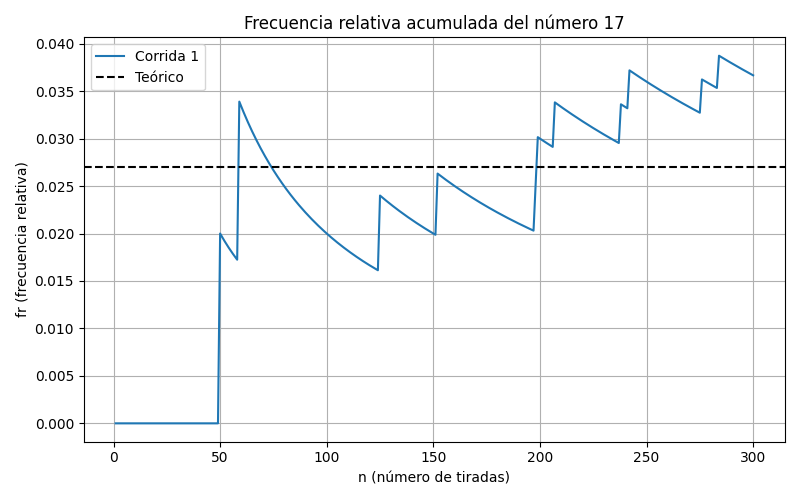
\includegraphics[width=0.5\textwidth]{Graficas/Frecuencia relativa 1C.png} &
    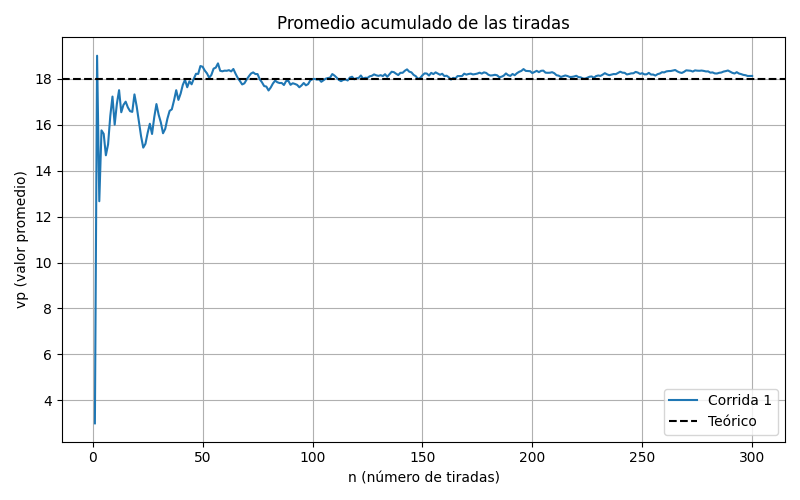
\includegraphics[width=0.5\textwidth]{Graficas/Promedio 1C.png} \\
    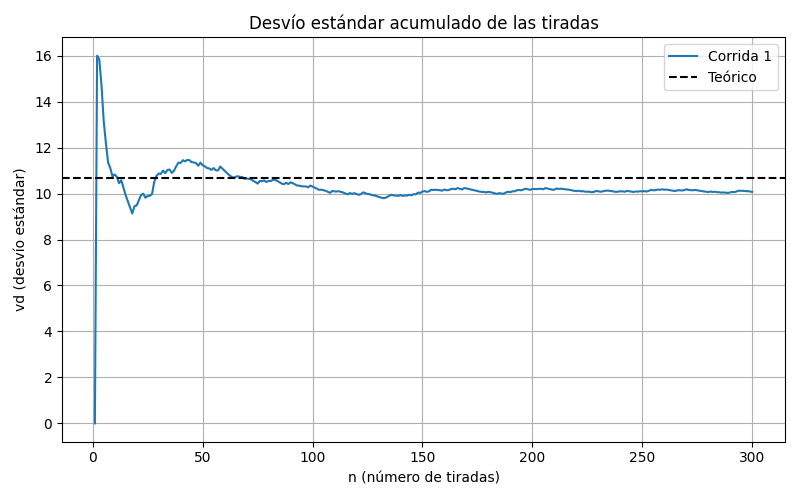
\includegraphics[width=0.5\textwidth]{Graficas/Desvio 1C.png} &
    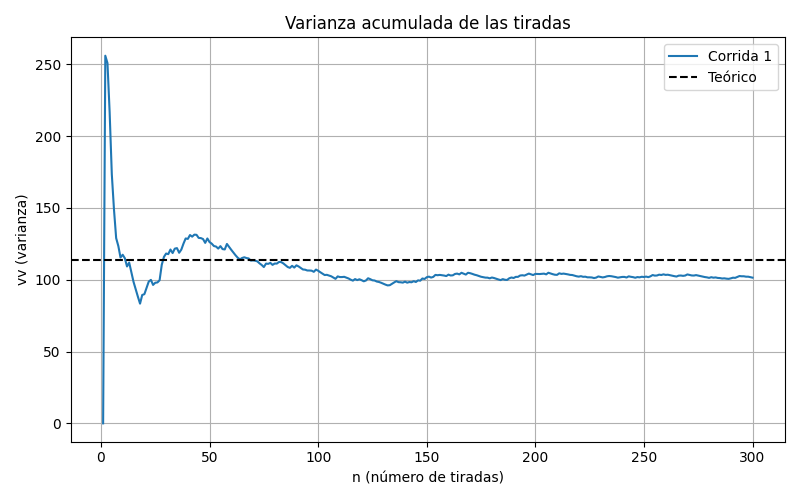
\includegraphics[width=0.5\textwidth]{Graficas/Varianza 1C.png} \\
  \end{tabular}
  \caption{Métricas estadísticas obtenidas con 1 corrida.}
\end{figure}

\begin{center}
    \item {Promedio de la corrida} 
        \begin{itemize}
          \item {Frecuencia relativa media: 0.0367}
          \item {Promedio medio: 18.1200}
          \item {Varianza media: 101.4523}
          \item {Desvío estándar medio: 10.0724}
        \end{itemize}
\end{center}


\subsection*{Resultados con 5 corridas, 300 tiradas, número elegido 17}

\begin{figure}[H]
  \centering
  \begin{tabular}{cc}
    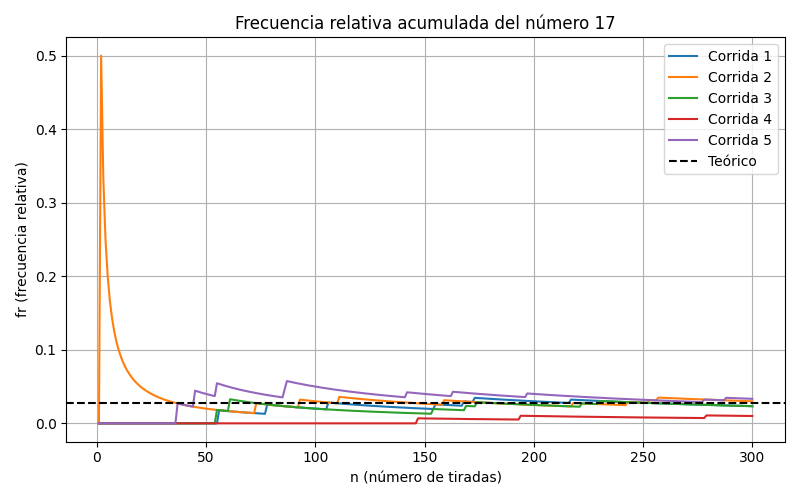
\includegraphics[width=0.5\textwidth]{Graficas/Frecuencia relativa 5C.png} &
    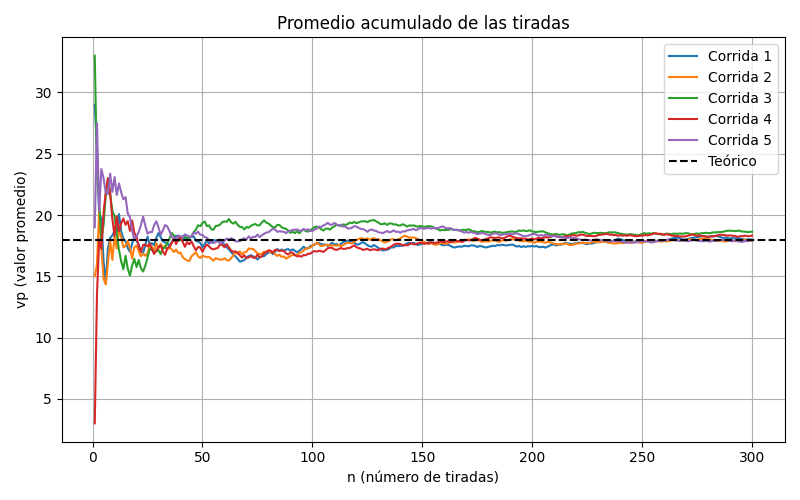
\includegraphics[width=0.5\textwidth]{Graficas/Promedio 5C.png} \\
     \\
    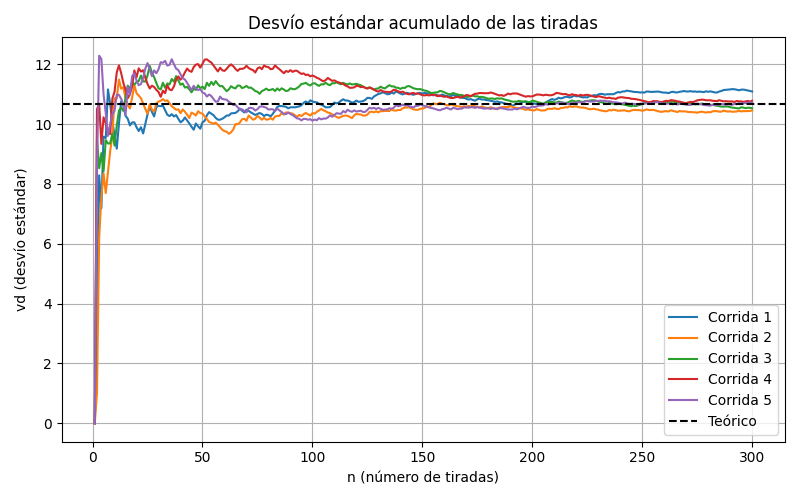
\includegraphics[width=0.5\textwidth]{Graficas/Desvio 5C.png} &
    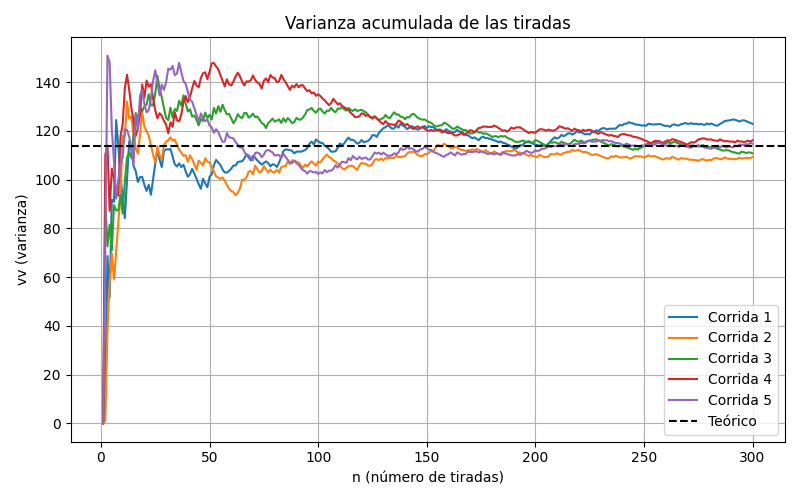
\includegraphics[width=0.5\textwidth]{Graficas/Varianza 5C.png} \\
    
  \end{tabular}
  \caption{Métricas estadísticas obtenidas con 5 corridas.}
\end{figure}

\begin{center}
    \item {Promedio entre todas las corridas}
        \begin{itemize}
          \item {Frecuencia relativa media: 0.0240}
          \item {Promedio medio: 18.1587}
          \item {Varianza media: 114.8086}
          \item {Desvío estándar medio: 10.7126}
        \end{itemize}
\end{center}


\subsection*{Resultados con 10 corridas, 300 tiradas cada una, número elegido 17}

\begin{figure}[H]
  \centering
  \begin{tabular}{cc}
    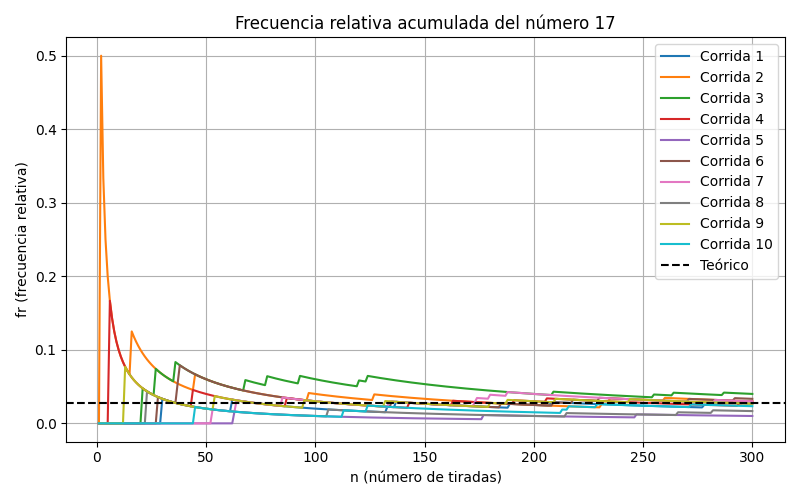
\includegraphics[width=0.45\textwidth]{Graficas/Frecuencia relativa 10C.png} &
    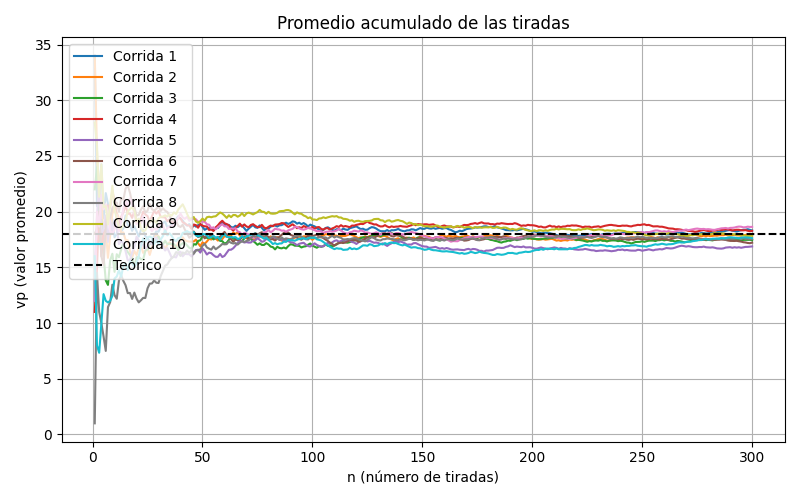
\includegraphics[width=0.45\textwidth]{Graficas/Promedio 10C.png} \\
    \textbf{Frecuencia relativa} & \textbf{Promedio acumulado} \\
    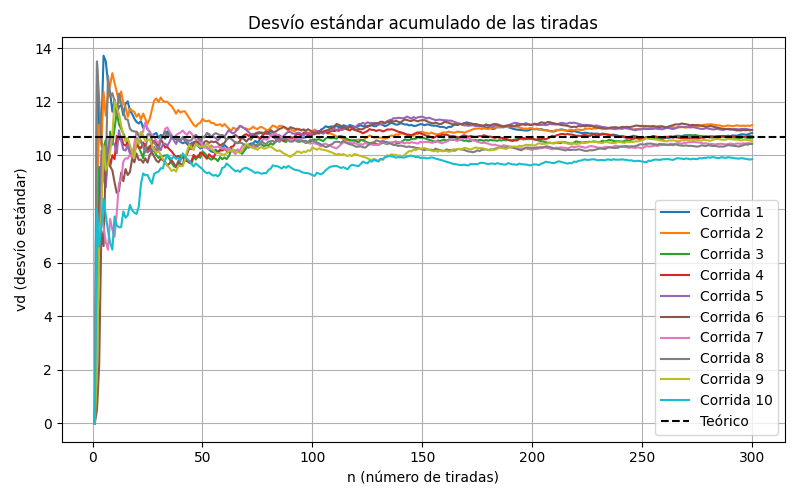
\includegraphics[width=0.45\textwidth]{Graficas/Desvio 10C.png} &
    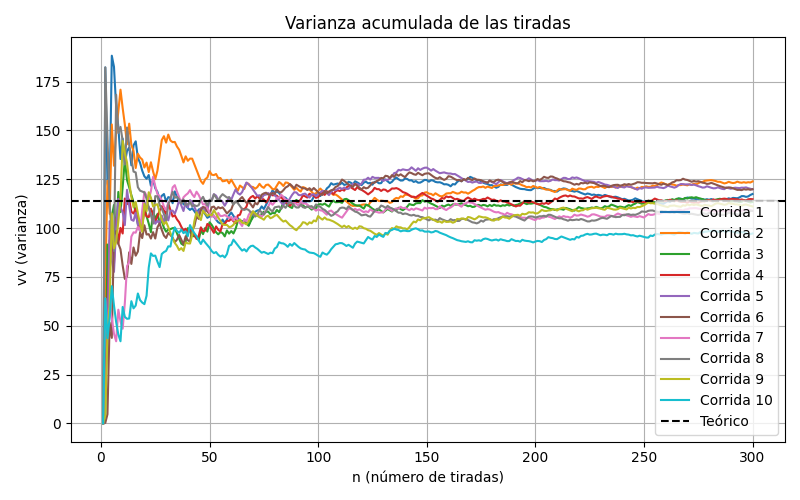
\includegraphics[width=0.45\textwidth]{Graficas/Varianza 10C.png} \\
    \textbf{Desvío estándar} & \textbf{Varianza acumulada}
  \end{tabular}
  \caption{Métricas estadísticas obtenidas con 10 corridas.}
\end{figure}

\begin{center}
    \item {Promedio entre todas las corridas}
        \begin{itemize}
          \item {Frecuencia relativa media: 0.0267}
          \item {Promedio medio: 17.7643}
          \item {Varianza media: 113.5056}
          \item {Desvío estándar medio: 10.6484}
        \end{itemize}
\end{center}

\subsection*{Resultados con 1 corrida, 10.000 tiradas cada una, número elegido 7}

\begin{figure}[H]
  \centering
  \begin{tabular}{cc}
    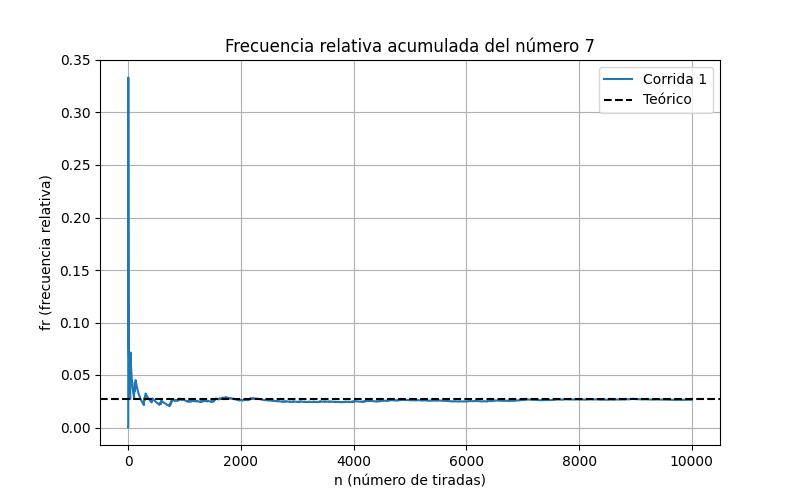
\includegraphics[width=0.45\textwidth]{Graficas/Frecuencia relativa 1C 10000T.png} &
    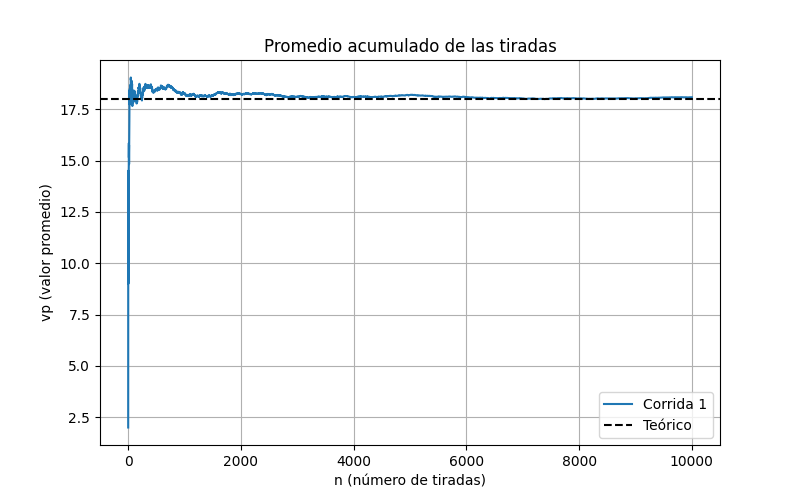
\includegraphics[width=0.45\textwidth]{Graficas/Promedio 1C 10000T.png} \\
    \textbf{Frecuencia relativa} & \textbf{Promedio acumulado} \\
    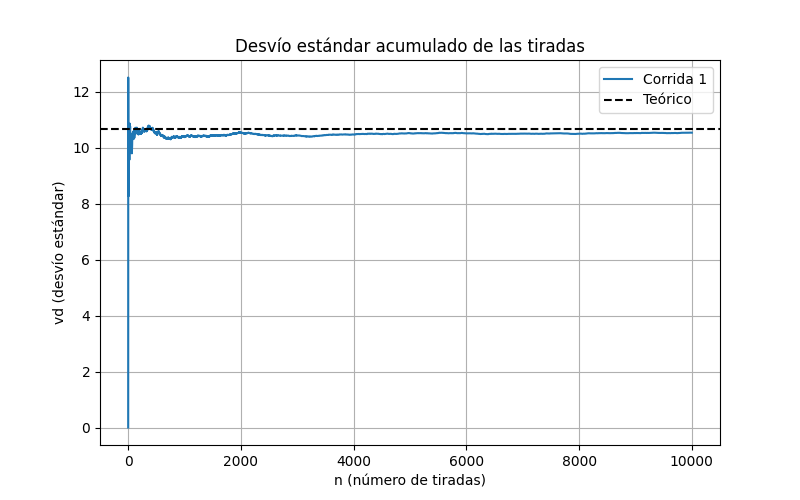
\includegraphics[width=0.45\textwidth]{Graficas/Desvio 1C 10000T.png} &
    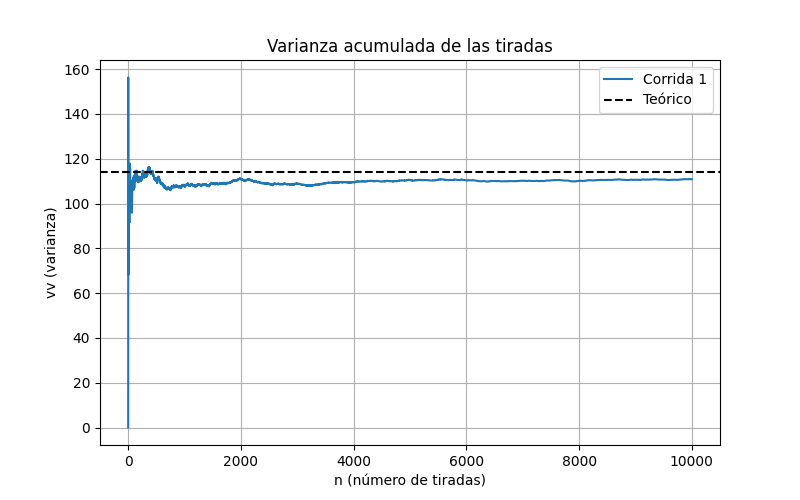
\includegraphics[width=0.45\textwidth]{Graficas/Varianza 1C 10000T.png} \\
    \textbf{Desvío estándar} & \textbf{Varianza acumulada}
  \end{tabular}
  \caption{Métricas estadísticas obtenidas con 1 corrida.}
\end{figure}

\begin{center}
    \item {Promedio entre todas las corridas}
        \begin{itemize}
          \item {Frecuencia relativa media: 0.0265}
          \item {Promedio medio: 18.0803}
          \item {Varianza media: 110.8613}
          \item {Desvío estándar medio: 10.5291}
        \end{itemize}
\end{center}

\subsection*{Resultados con 5 corridas, 10.000 tiradas cada una, número elegido 7}

\begin{figure}[H]
  \centering
  \begin{tabular}{cc}
    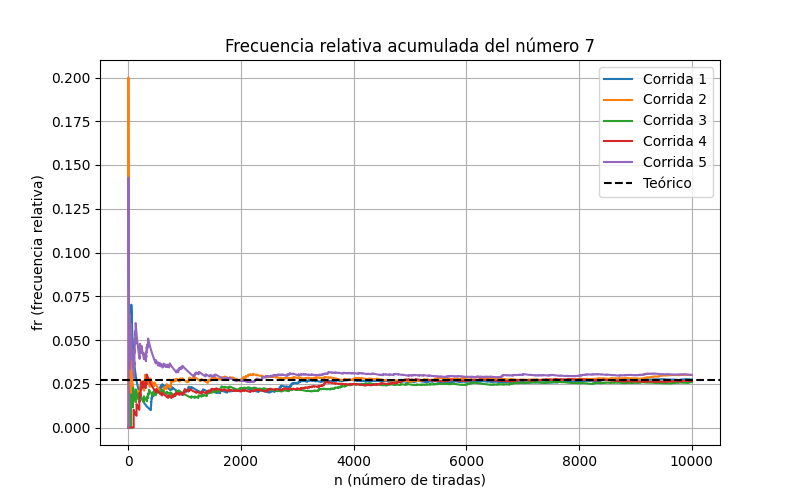
\includegraphics[width=0.45\textwidth]{Graficas/Frecuencia relativa 5C 10000T.png} &
    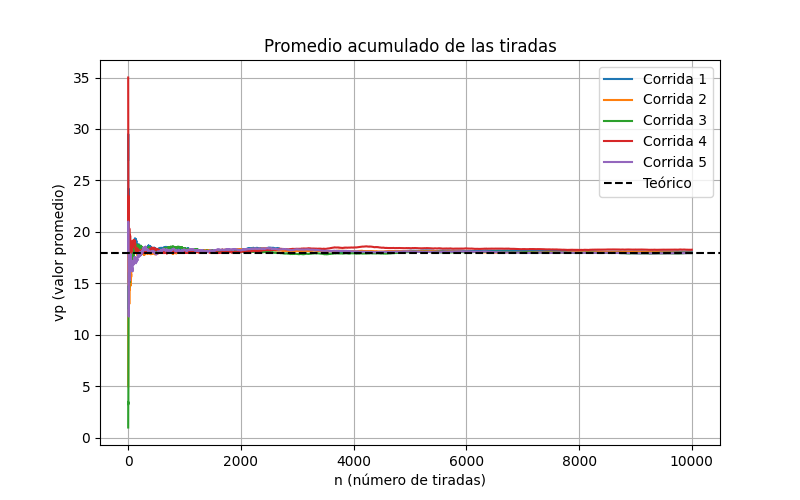
\includegraphics[width=0.45\textwidth]{Graficas/Promedio 5C 10000T.png} \\
    \textbf{Frecuencia relativa} & \textbf{Promedio acumulado} \\
    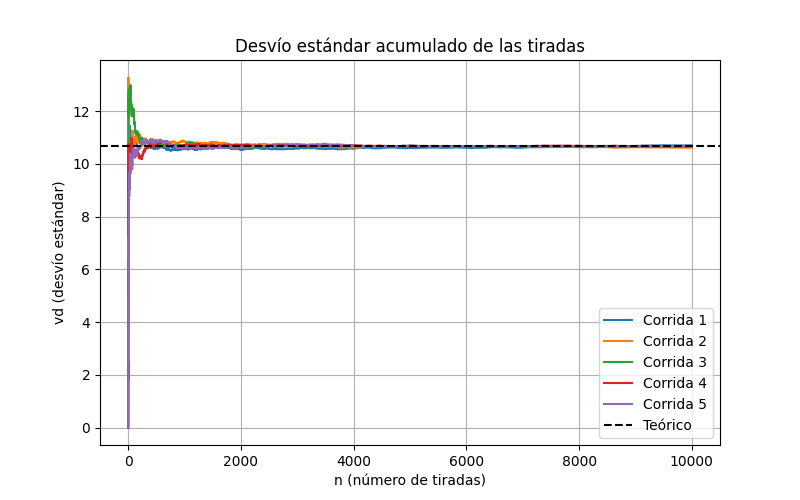
\includegraphics[width=0.45\textwidth]{Graficas/Desvio 5C 10000T.png} &
    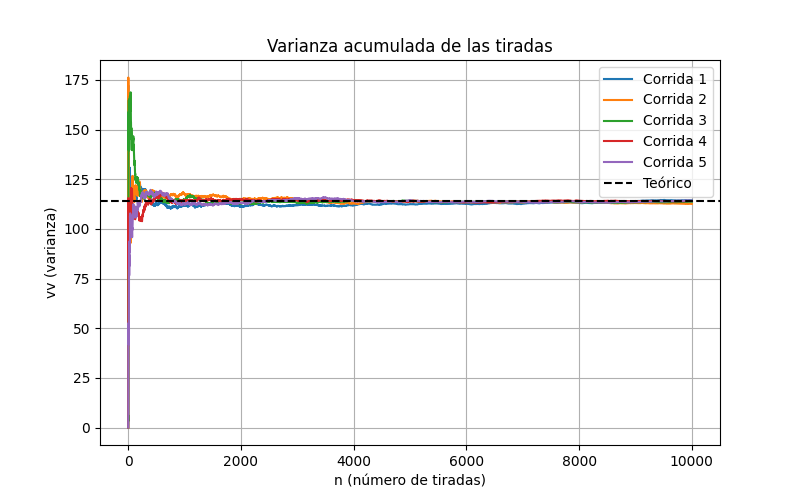
\includegraphics[width=0.45\textwidth]{Graficas/Varianza 5C 10000T.png} \\
    \textbf{Desvío estándar} & \textbf{Varianza acumulada}
  \end{tabular}
  \caption{Métricas estadísticas obtenidas con 5 corridas.}
\end{figure}

\begin{center}
    \item {Promedio entre todas las corridas}
        \begin{itemize}
          \item {Frecuencia relativa media: 0.0280}
          \item {Promedio medio: 18.0469}
          \item {Varianza media: 113.7254}
          \item {Desvío estándar medio: 10.6642}
        \end{itemize}
\end{center}

\subsection*{Resultados con 10 corridas, 10.000 tiradas cada una, número elegido 7}

\begin{figure}[H]
  \centering
  \begin{tabular}{cc}
    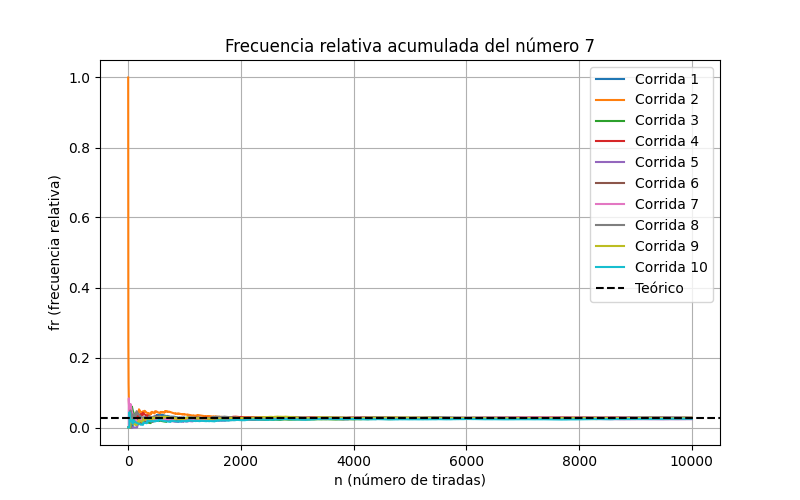
\includegraphics[width=0.45\textwidth]{Graficas/Frecuencia relativa 10C 10000T.png} &
    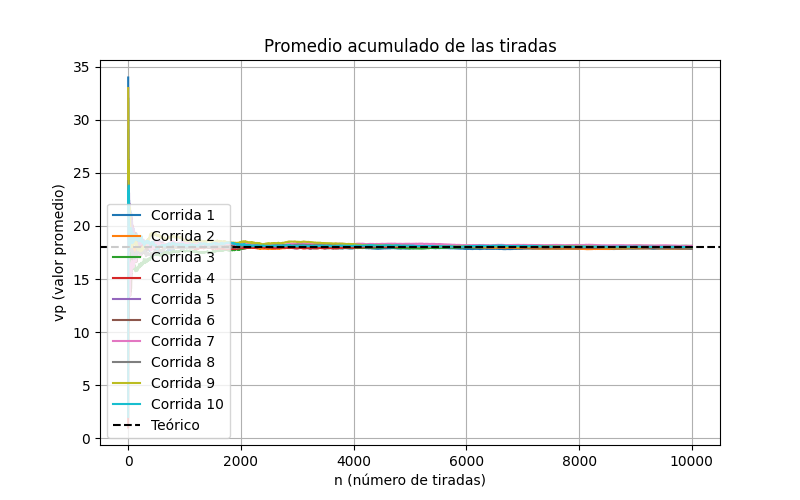
\includegraphics[width=0.45\textwidth]{Graficas/Promedio 10C 10000T.png} \\
    \textbf{Frecuencia relativa} & \textbf{Promedio acumulado} \\
    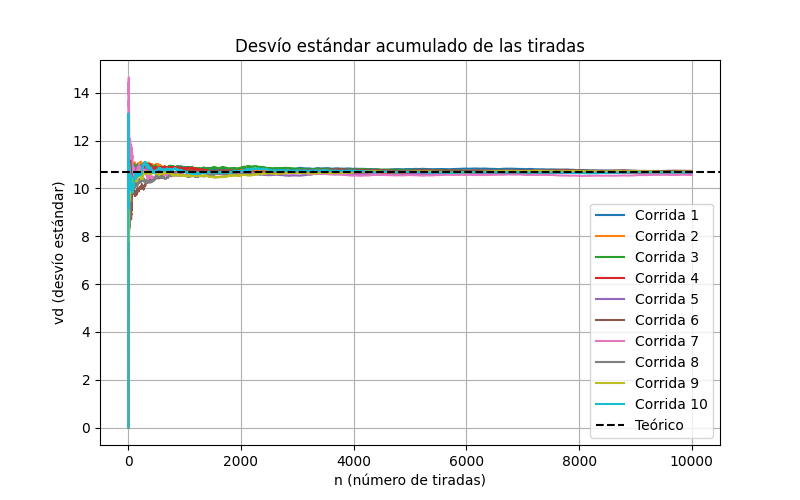
\includegraphics[width=0.45\textwidth]{Graficas/Desvio 10C 10000T.png} &
    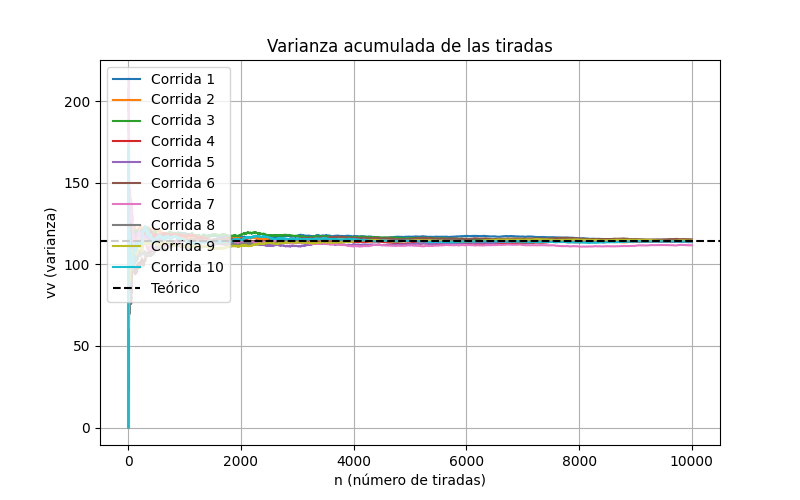
\includegraphics[width=0.45\textwidth]{Graficas/Varianza 10C 10000T.png} \\
    \textbf{Desvío estándar} & \textbf{Varianza acumulada}
  \end{tabular}
  \caption{Métricas estadísticas obtenidas con 10 corridas.}
\end{figure}

\begin{center}
    \item {Promedio entre todas las corridas}
        \begin{itemize}
          \item {Frecuencia relativa media: 0.0263}
          \item {Promedio medio: 17.8423}
          \item {Varianza media: 115.1215}
          \item {Desvío estándar medio: 10.7285}
        \end{itemize}
\end{center}

\subsection*{Histogramas de fracuencias absolutas}
\begin{figure}[H]
  \centering
  \begin{tabular}{cc}
    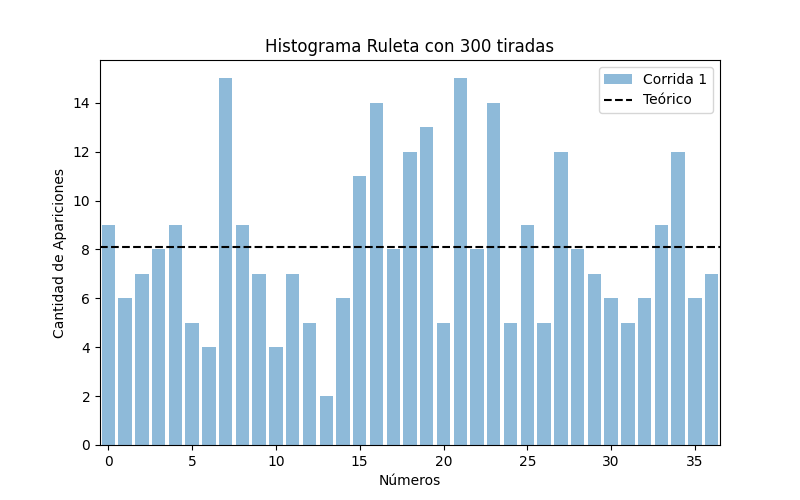
\includegraphics[width=0.45\textwidth]{Graficas/Histograma 1C.png} &
    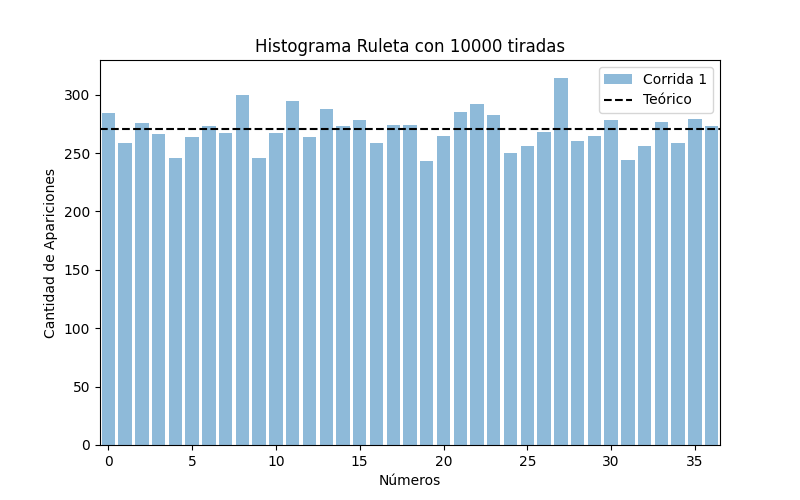
\includegraphics[width=0.45\textwidth]{Graficas/Histograma 1C 10000T.png} \\
    \textbf{1 corrida, 300 tiradas} & \textbf{1 corridas, 10.000 tiradas}
  \end{tabular}
  \caption{Histogramas de frecuencias absolutas de los resultados obtenidos en las simulaciones con una corrida.}
\end{figure}
\begin{figure}[H]
  \centering
  \begin{tabular}{cc}
    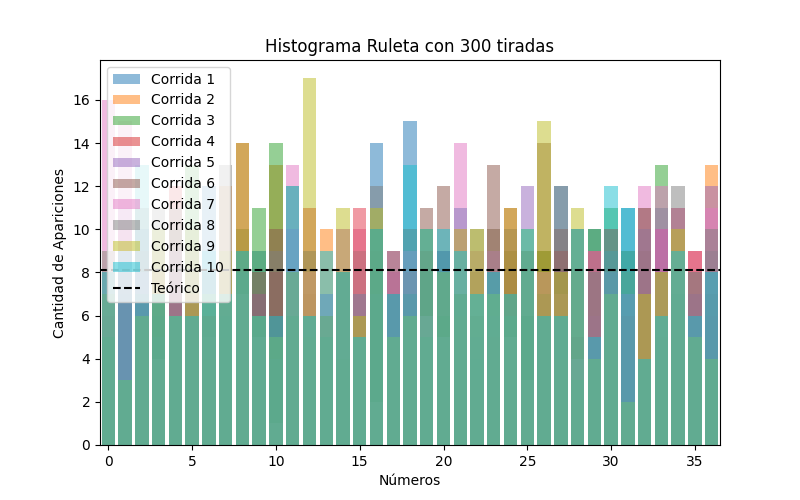
\includegraphics[width=0.45\textwidth]{Graficas/Histograma 10C.png} &
    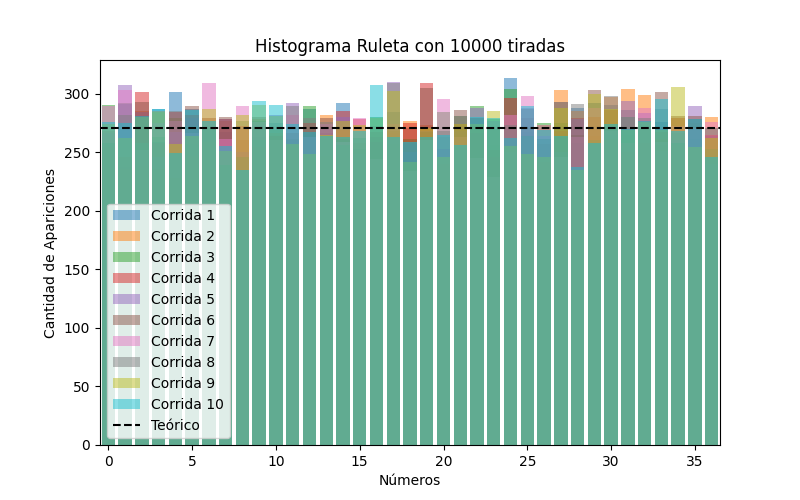
\includegraphics[width=0.45\textwidth]{Graficas/Histograma 10C 10000T.png} \\
    \textbf{10 corrida, 300 tiradas} & \textbf{10 corridas, 10.000 tiradas}
  \end{tabular}
  \caption{Histogramas de los resultados obtenidos en las simulaciones con diez corridas.}
\end{figure}

\subsection*{Histogramas de promedios de las medias muestrales}
\begin{figure}[H]
  \centering
  \begin{tabular}{cc}
    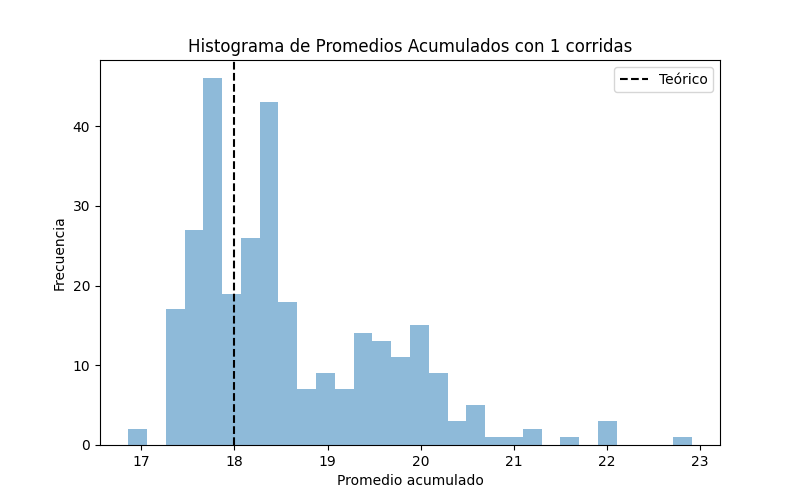
\includegraphics[width=0.45\textwidth]{Graficas/Histograma_Promedios 1C.png} &
    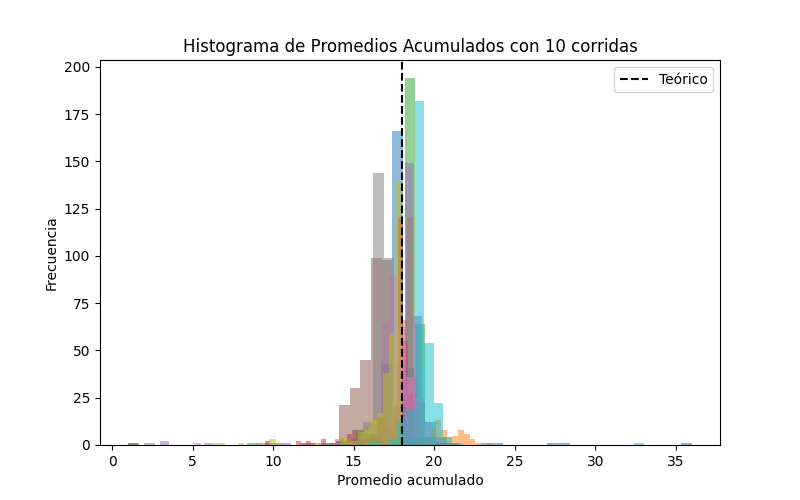
\includegraphics[width=0.45\textwidth]{Graficas/Histograma_Promedios 10C.png} \\
    \textbf{1 corrida, 300 tiradas} & \textbf{10 corridas, 300 tiradas}
  \end{tabular}
  \caption{Histogramas de los promedios de las medias muestrales obtenidos en las simulaciones con una y diez corridas con 300 tiradas cada una.}
\end{figure}
\begin{figure}
  \centering
  \begin{tabular}{cc}
    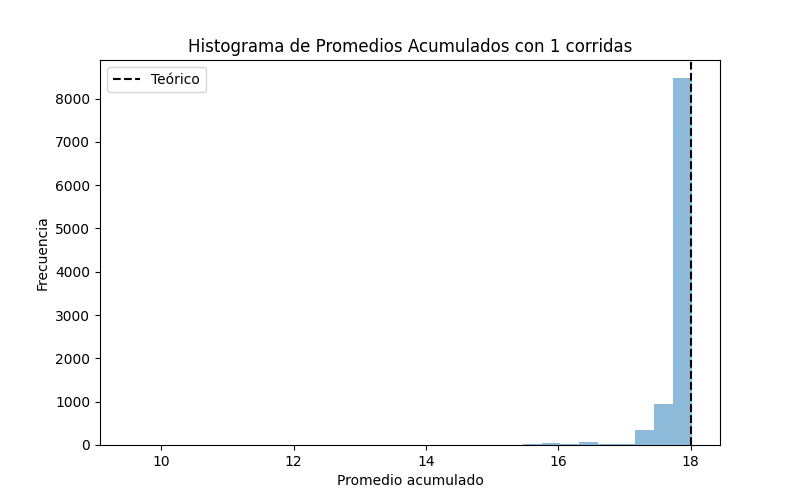
\includegraphics[width=0.45\textwidth]{Graficas/Histograma_Promedios 1C 10000T.png} &
    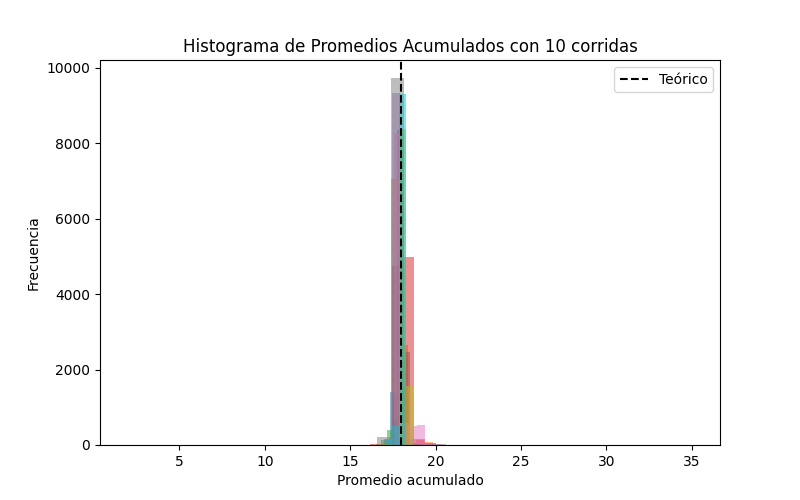
\includegraphics[width=0.45\textwidth]{Graficas/Histograma_Promedios 10C 10000T.png} \\
    \textbf{1 corrida, 10.000 tiradas} & \textbf{10 corridas, 10.000 tiradas}
  \end{tabular}
  \caption{Histogramas de los promedios de las medias muestrales obtenidos en las simulaciones con una y diez corridas con 10.000 tiradas cada una.}
\end{figure}

\section{Discusión}

El análisis de las simulaciones permite observar una clara diferencia entre el comportamiento aleatorio de las ejecuciones a corto plazo y la estabilidad a largo plazo. Teniendo en cuenta los resultados pueden destacarse los siguientes hallazgos:

\subsection{Análisis de Volatilidad y Convergencia}
Comenzando por las simulaciones con bajo nivel de observaciones ($N=300$), se observa una alta volatilidad en las métricas. En la \textbf{figura 1} la frecuencia relativa y el promedio muestran un comportamiento errático durante las primeras 100 tiradas, lo cual es consistente con lo esperado de pequeñas muestras con alta sensibilidad a lo aleatorio que no logran ser representativas de la población.

Por el contrario, al contar con simulaciones donde se incrementa el número de tiradas hacia valores muy altos ($N=10.000$), podemos observar en la \textbf{figura 6} una estabilización en las curvas de cada corrida hacia los valores teóricos esperados. Este comportamiento cumple como validación de la Ley de Grandes Números, donde la repetición en cantidad de un experimento, logra que el promedio experimental converge al promedio teórico.

\subsection{Interpretación de los Histogramas de Frecuencia}
Los histogramas de frecuencias absolutas de las \textbf{figuras 7 y 8} permiten observar gráficamente la naturaleza de la distribución uniforme que presenta la ruleta.
Al contar con un bajo número de tiradas ($N=300$) las barras presentan variaciones en sus alturas, lo que puede ser erróneamente interpretado como sesgos por algunos números, pero al aumentar en gran cantidad las observaciones, las barras se nivelan aproximandosé a la línea teórica de la equiprobabilidad ($1/37$).

\subsection{Interpretación de los Histogramas relacionados al Teorema Central del Límite}
Los histogramas de promedios de las medias muestrales de las \textbf{figura 9 y 10} son fundamentales para observar cómo a pesar de que los resultados individuales de la ruleta siguen una distribución uniforme, la distribución de sus promedios acumulados de múltiples corridas adopta una forma acampanada característica de la distribución normal.

Al comparar las simulaciones de 1 corrida frente a las de 10 corridas, se observa que la dispersión de las medias disminuye y se concentra con mayor precisión en torno al valor teórico de 18. Este fenómeno es una demostración directa del Teorema Central del Límite, el cual postula que la distribución de las medias muestrales tenderá a la normalidad independientemente de la distribución de la población original.

\section{Conclusión}

A lo largo del trabajo se pudo observar que, a medida que aumentamos la cantidad de tiradas, los valores de las métricas estadísticas —como la frecuencia relativa, el promedio, la varianza y la desviación estándar— se vuelven cada vez más estables y se acercan a los valores que uno esperaría teóricamente en una ruleta justa. Al comparar los histogramas de frecuencia absoluta de las diferentes ejecuciones del programa, se observa con facilidad cómo, a mayor cantidad de tiradas y corridas, la concurrencia de cada número de la ruleta se asienta en el teórico esperado. Esto confirma, de forma simple y visual, la conocida \textbf{ley de los grandes números}: la repetición en cantidad de un experimento logra que el promedio experimental converja al promedio teórico, diluyendo la variabilidad aleatoria a gran escala.

El promedio de las tiradas tendió a estabilizarse en torno al valor esperado de $18$ , mientras que la varianza y el desvío estándar se aproximaron a los valores teóricos de una distribución uniforme discreta en el rango $[0, 36]$. Las variaciones observadas en pequeñas muestras demuestran el azar en el corto plazo, pero este se estabiliza a largo plazo con muestras más grandes y representativas. Además, al ejecutar el programa con diferentes cantidades de corridas (1, 5 y 10), se nota que aunque el comportamiento general de las simulaciones es parecido, existen pequeñas variaciones entre cada corrida. Esto refleja el carácter aleatorio del experimento, pero también muestra que a mayor cantidad de corridas, el resultado promedio se vuelve más confiable.
 
Por último, se demostró el Teorema Central del Límite mediante el análisis de los histogramas de medias muestrales, donde se observó cómo la distribución de los promedios tiende a una distribución normal, lo que incrementa la confiabilidad del resultado.

Este tipo de simulaciones con Python resulta muy útil y robusto para estudiar cómo se comportan los procesos aleatorios y cómo evolucionan sus estadísticas a lo largo del tiempo.

\section{Referencias}
\begin{itemize}
  \item Wikipedia. \textit{Ruleta}. https://es.wikipedia.org/wiki/Ruleta
  \item Cornell University LaTeX Template. https://es.overleaf.com/latex/templates/style-and-template-for-preprints-arxiv-bio-arxiv/pkzcrhzcdxmc
  \item ReLópez-Briega. \textit{Probabilidad y estadística con Python}. https://relopezbriega.github.io/blog/2015/06/27/probabilidad-y-estadistica-con-python/
  \item Python para impacientes. https://python-para-impacientes.blogspot.com/2014/08/graficos-en-ipython.html
  \item Documentación oficial de Matplotlib. https://matplotlib.org/stable/users/index
\end{itemize}

\end{document}